\question Em um estudo sobre contusões causadas durante a prática de esportes, 25 escolas de um estado brasileiro foram selecionadas, ao acaso, entrevistadas. Foram coletados os dados abaixo, sobre o número de contusões classificadas como graves em atletas do sexo masculino para duas modalidades de esporte.
\begin{parts}
    \part Construa uma distribuição de frequências para as 50 observações.
    \begin{solution}
        % latex table generated in R 4.3.3 by xtable 1.8-4 package
        % Sun Mar 17 17:29:18 2024
        \begin{table}[H]
            \centering
            \begin{tabular}{rlr}
                \hline
                  & Num. Contusões & Freq \\
                \hline
                1 & 1              & 8    \\
                2 & 2              & 8    \\
                3 & 3              & 7    \\
                4 & 4              & 6    \\
                5 & 5              & 7    \\
                6 & 6              & 7    \\
                7 & 7              & 7    \\
                \hline
            \end{tabular}
        \end{table}
    \end{solution}
    \part Construa uma distribuição de frequências para cada modalidade.
    \begin{solution}
        % latex table generated in R 4.3.3 by xtable 1.8-4 package
        % Sun Mar 17 17:39:57 2024
        \begin{table}[H]
            \centering
            \begin{tabular}{rlr}
                \hline
                  & Basquete              \\
                \hline
                  & Num. Contusões & Freq \\
                \hline
                1 & 1              & 1    \\
                2 & 2              & 4    \\
                3 & 3              & 5    \\
                4 & 4              & 6    \\
                5 & 5              & 5    \\
                6 & 6              & 3    \\
                7 & 7              & 1    \\
                \hline
            \end{tabular}
        \end{table}
        % latex table generated in R 4.3.3 by xtable 1.8-4 package
        % Sun Mar 17 17:39:48 2024
        \begin{table}[H]
            \centering
            \begin{tabular}{rlr}
                \hline
                  & Futebol               \\
                \hline
                  & Num. Contusões & Freq \\
                \hline
                1 & 1              & 7    \\
                2 & 2              & 4    \\
                3 & 3              & 2    \\
                4 & 5              & 2    \\
                5 & 6              & 4    \\
                6 & 7              & 6    \\
                \hline
            \end{tabular}
        \end{table}
    \end{solution}
    \pagebreak
    \part Represente graficamente cada uma das distribuições.
    \begin{solution}
        Para ambos a variável de interesse é uma \textbf{variável quantitativa discreta}, Assim a melhor forma de representar graficamente é por meio de um \textbf{gráfico de colunas}.
        \begin{figure}[H]
            \centering
            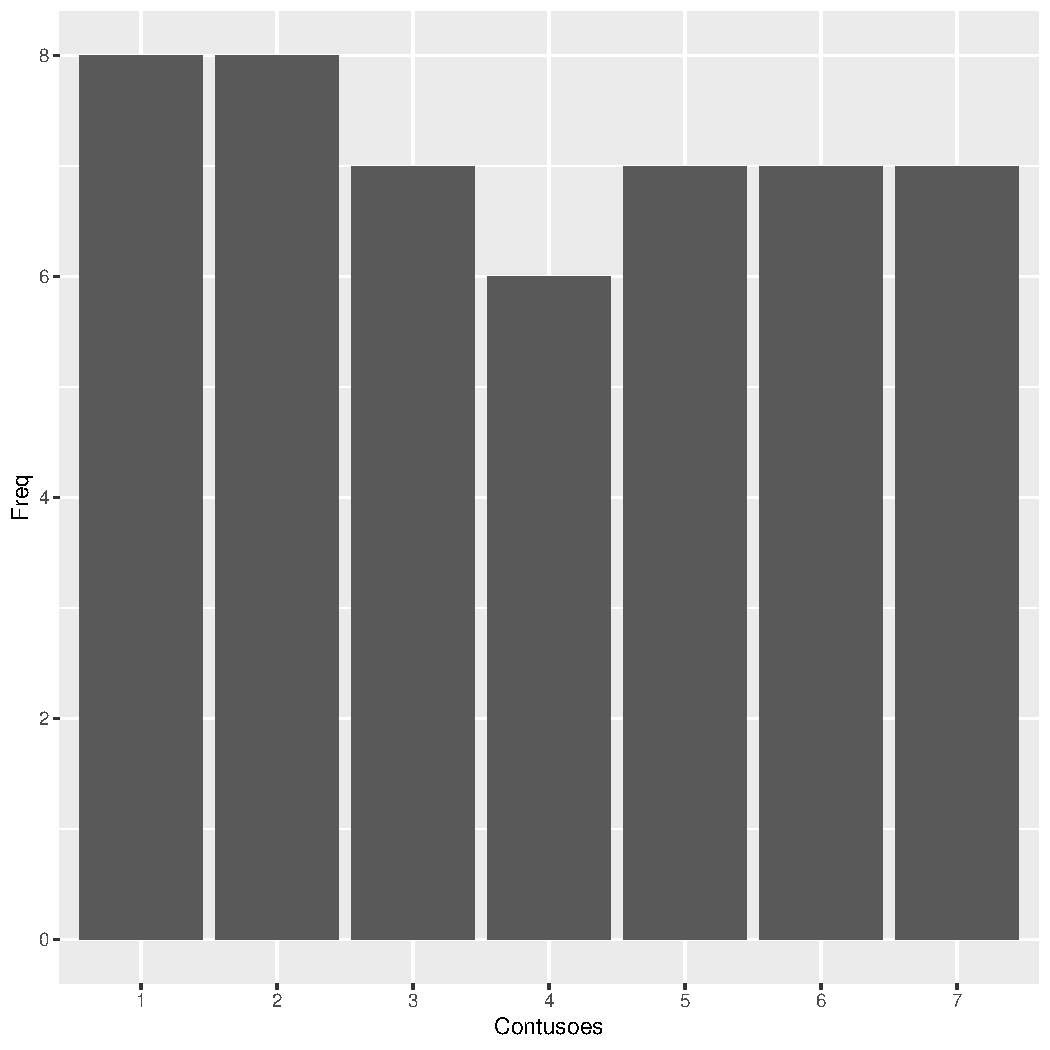
\includegraphics[width=8cm]{./assets/03172024_Plot_ContusoesMerged.pdf}
            \caption[short]{Contusões no Basquete e Futebol}
        \end{figure}
        \begin{figure}[H]
            \centering
            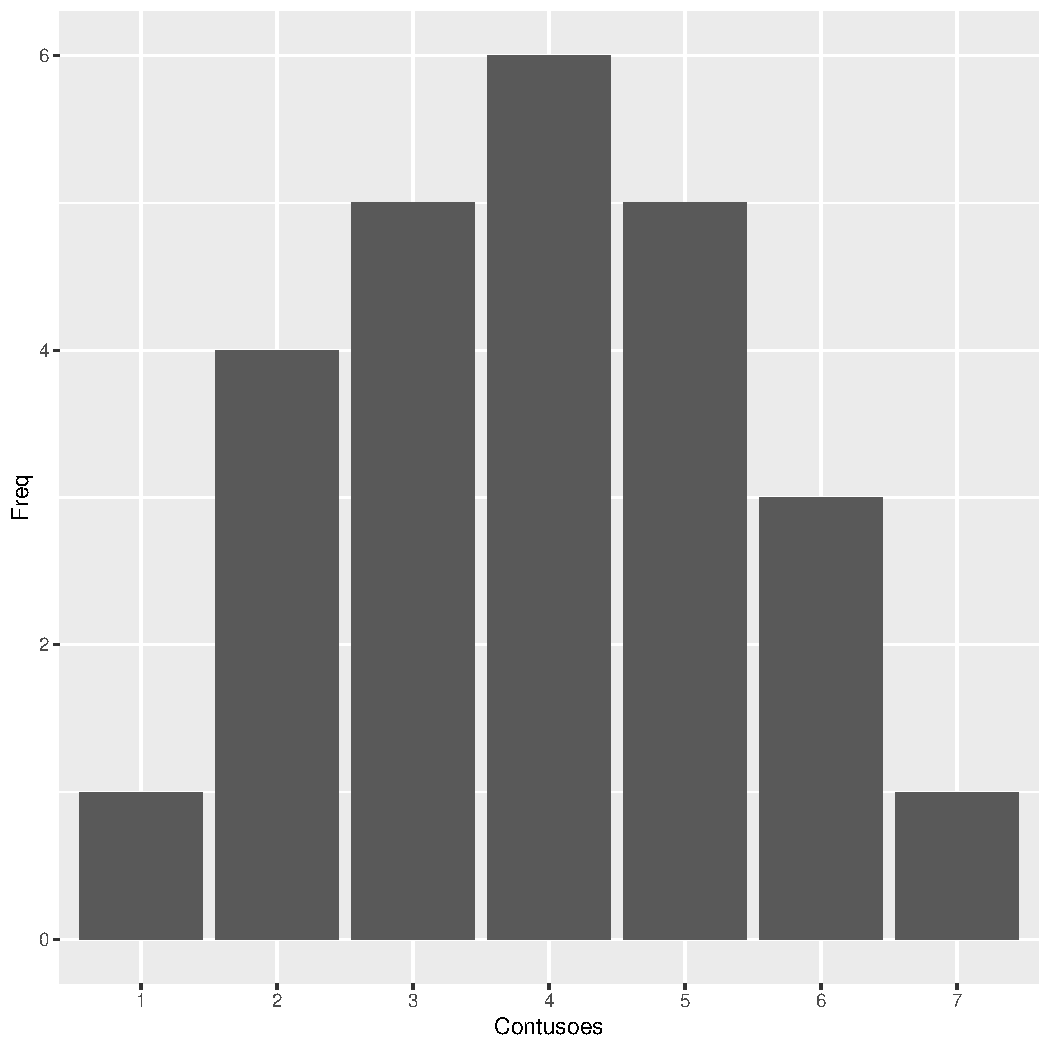
\includegraphics[width=8cm]{./assets/03172024_Plot_ContusoesBasquete.pdf}
            \caption[short]{Contusões no Basquete}
        \end{figure}
        \begin{figure}[H]
            \centering
            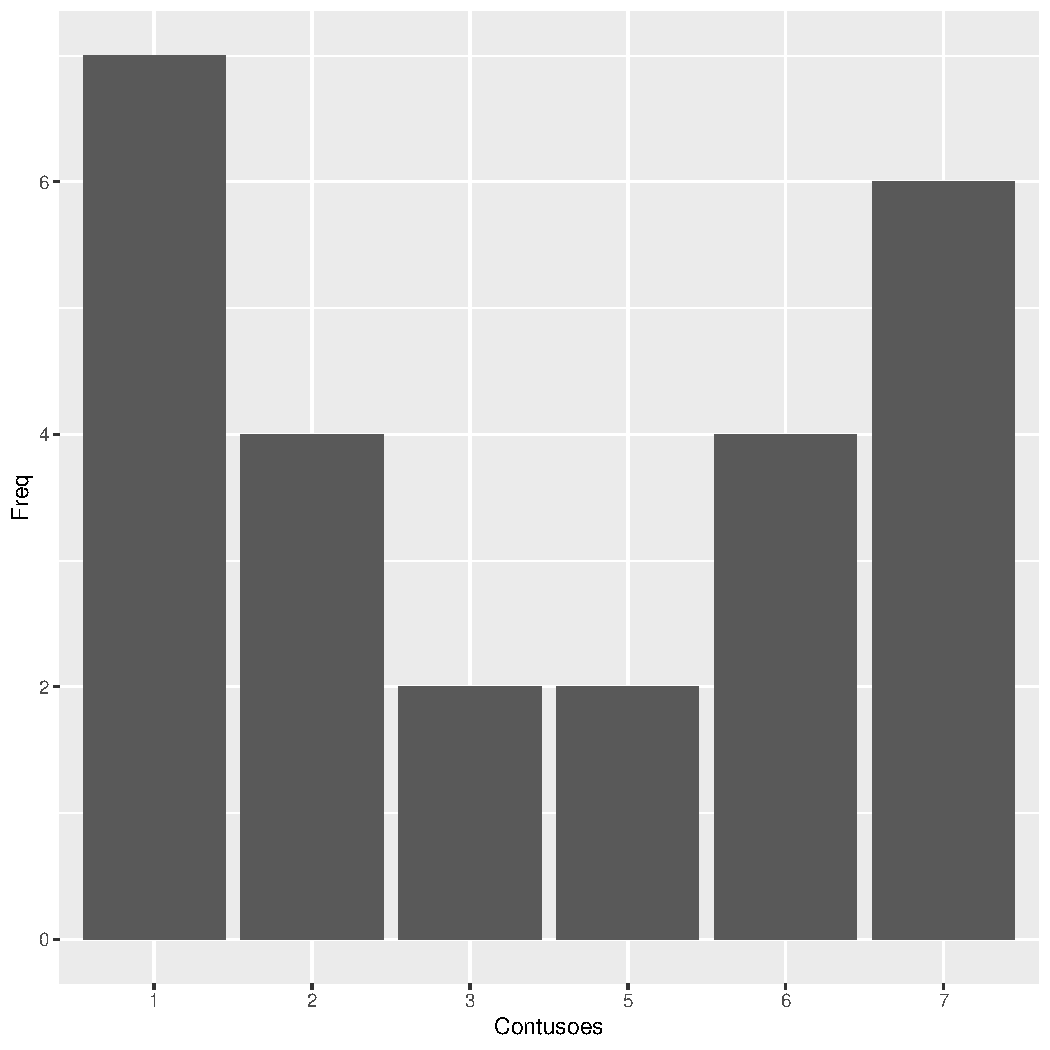
\includegraphics[width=8cm]{./assets/03172024_Plot_ContusoesFutebol.pdf}
            \caption[short]{Contusões no Futebol}
        \end{figure}
    \end{solution}
    \part Comente os resultados.
    \begin{solution}
        Percebe-se que a distribuição das contusões no basquete é inferior nos extremos e maior em valores medianos, diferentemente do futebol.
    \end{solution}
\end{parts}